% =============================================================================
% 2. INTRODUCTION
% =============================================================================

\begin{figure}[h!]
\centering
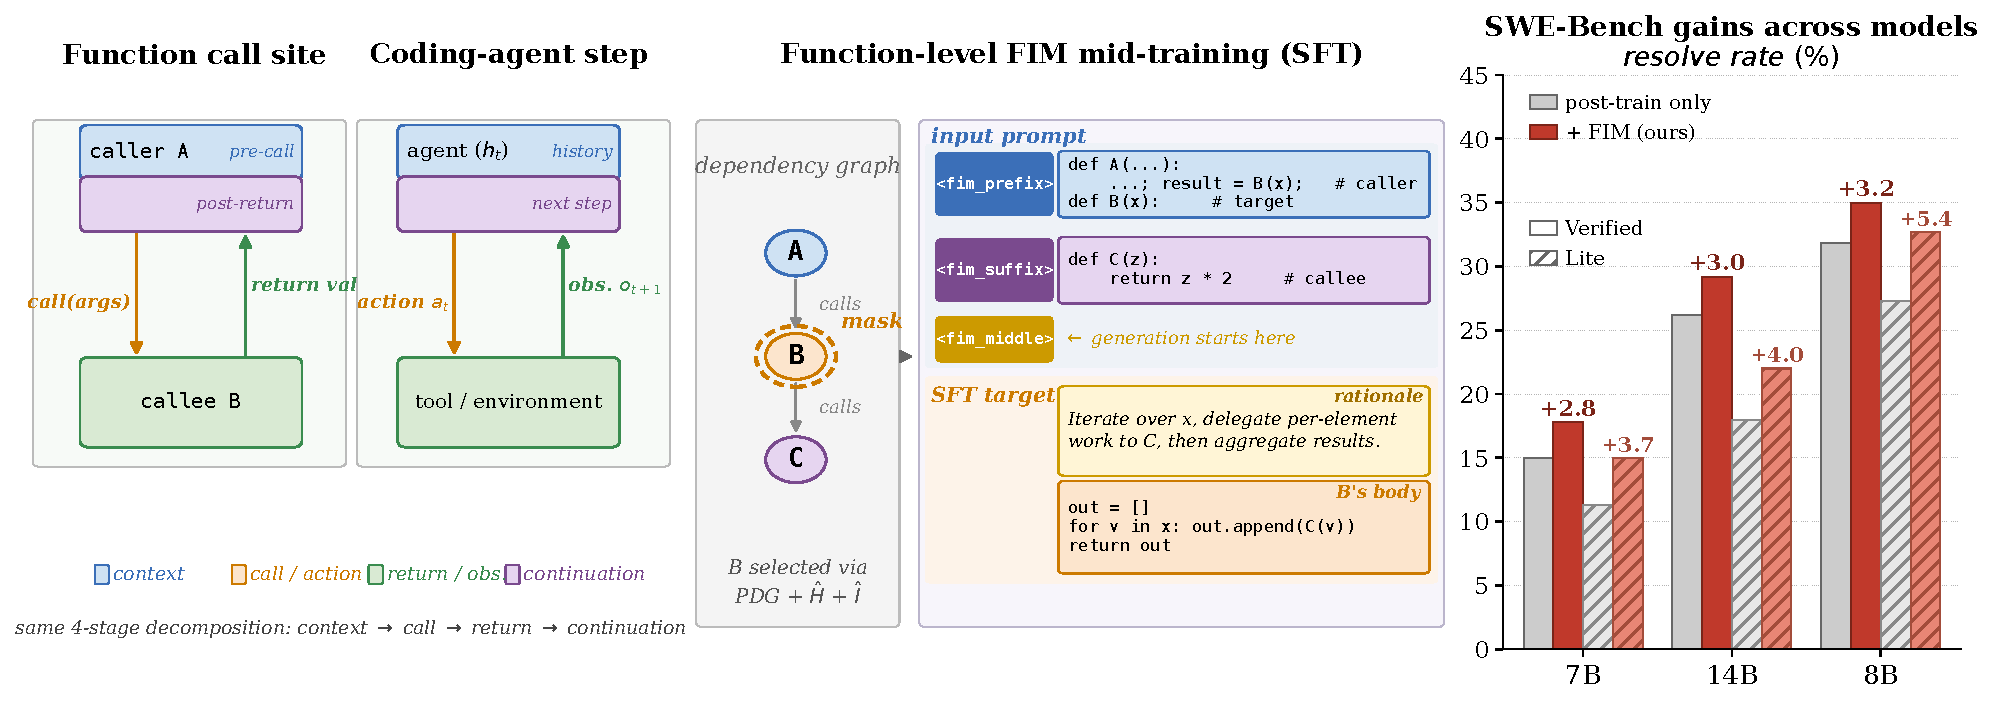
\includegraphics[width=\linewidth]{figs/teaser_v34.pdf}

\vspace{-1.9ex}
\caption{%
\textbf{Left:} A function call site and a single step of a coding agent
are \emph{structurally similar}, decomposing into the
same four stages: context, call/action, return/observation, continuation.
\textbf{Middle:} We exploit this analogy via function-aware FIM
mid-training. A function $B$ is selected from the program dependency
graph using complexity ($\hat{H}$) and inferability ($\hat{I}$) scores;
the model is then mid-trained to fill in $B$'s body together with a
chain-of-thought rationale, given the surrounding file as an
FIM-formatted prompt.
\textbf{Right:} Mid-training yields consistent gains across both Qwen2.5-Coder (7B, 14B) and Qwen3 (8B) on SWE-Bench-Verified (solid bars) and SWE-Bench-Lite (hatched bars).}
\vspace{-1.5ex}
\label{fig:teaser}
\end{figure}

\section{Introduction}
\label{sec:intro}

Coding agents that resolve real software engineering issues have moved from
research demos to deployed systems~\citep{swebench, sweagent,
openhands}. Their progress, however, has been driven almost entirely by
scaling synthetic agent-trajectory data during post-training: pipelines such
as SWE-Gym~\citep{swegym}, R2E-Gym~\citep{r2egym}, and
SWE-Smith~\citep{swesmith} curate or synthesize trajectories that
imitate human or LLM behavior on issue-resolution tasks. The base model
these pipelines start from is typically a code LLM trained with next-token
prediction (and, in some cases, random-span FIM) on internet-scale
code~\citep{qwencoder, deepseekcoder, starcoder}. Between
these two stages lies a training-time gap: the base model is rarely
optimized for the conditioning structure that agentic post-training will
later demand. We treat this gap as an opportunity for a dedicated
\emph{mid-training} stage that aligns the base model with agent-relevant
inductive biases before agent-specific data is introduced.

Our central observation is that the inductive bias required by a coding
agent already exists in ordinary code, but in a shape that left-to-right
pretraining systematically under-exposes. At each step an agent maintains a
history $h_t$, samples an action $a_t \sim \pi(a_t \mid h_t)$, receives an
observation $o_{t+1}$ produced by an external process, and continues
conditioned on the entire trace. This four-part decomposition---context,
action, externally-computed return, continuation---is precisely the
decomposition of a function call site: pre-call code that establishes intent
and binds arguments; the call itself; a return value produced by code
outside the immediate scope; and downstream code that consumes the return
value (Figure~\ref{fig:teaser}, left). A model trained to reason
\emph{bidirectionally} about function-level dependencies must learn to
reconstruct a callee's behavior from caller context and downstream usage,
which is the same competence required to predict an agent's continuation
given a history and a tool return. The correspondence is structural rather
than literal---FIM training conditions on a given suffix while agent
inference generates one---but it suggests that representations induced by
the former should transfer to the latter, an empirical question we address
in Section~\ref{sec:exp}.

The fill-in-the-middle objective is not new~\citep{bavarian2022fim};
recent code LLMs mix random-span FIM into pretraining~\citep{qwencoder,
deepseekcoder, starcoder}. Random-span FIM is nonetheless poorly aligned
with agentic conditioning for three reasons. \emph{(i) Span boundaries
are syntactically arbitrary:} most masked spans cut through expressions
or partial statements and carry weak signal about function-level
dependencies. \emph{(ii) There is no reasoning supervision:} the model
fills the span directly, with no intermediate rationale mirroring an
agent's think-then-act pattern. \emph{(iii) The objective is dissolved
into pretraining:} by the time post-training begins, any structural prior
conferred by FIM has been amortized across trillions of unrelated tokens.
We address all three points: masking targets are selected at function
granularity using program dependency graph analysis with a
complexity--inferability double criterion that is deliberately
base-model-agnostic (Section~\ref{sec:method:selection}); chain-of-thought
rationales are embedded \emph{inside} the FIM middle span so the model
produces reasoning consistent with the eventual code
(Section~\ref{sec:method:cot}); and the objective is applied at a
dedicated mid-training stage, concentrating its signal immediately before
agentic post-training.

We evaluate this recipe along three axes of robustness. \emph{On the
Qwen2.5-Coder-Instruct series}, mid-training improves SWE-Bench-Verified
by $+2.8$ and $+3.0$ points at 7B and 14B respectively, indicating that
the structural prior is not absorbed by larger pretrained models in the
practical deployment range. \emph{Across two post-training pipelines},
mid-training improves both R2E-Gym and SWE-Smith on the same 7B base,
with the SWE-Smith pairing yielding $+5.3$ points on SWE-Bench-Verified.
\emph{On a non-Qwen2.5 base}, mid-training transfers to Qwen3-8B (paired
with SWE-Lego) for a $+3.2$-point gain on SWE-Bench-Verified; this single
comparison varies the post-training pipeline jointly with the base model
and should be read as evidence that the prior is not specific to a single
Qwen2.5-Coder $+$ R2E-Gym/SWE-Smith combination, rather than as a
guarantee across families.

A second set of results probes our motivating hypothesis. All checkpoints
are evaluated after the full pipeline (post-training alone, or
mid-training followed by post-training), since FIM-only checkpoints
degrade instruction-following and are not comparable to instruction-tuned
baselines. Agentic post-training alone substantially regresses non-target
capabilities at 14B, dropping LiveCodeBench, BFCL, and $\tau$-bench by
double-digit margins in some cases; adding mid-training before the same
post-training restores $+11.1$ on LiveCodeBench, $+2.4$ on BFCL, and
$+3.9$ on $\tau$-bench. Since the mid-training corpus contains only
Python code with no tool-use data, the cross-domain recovery is direct
evidence for the function-call/tool-call isomorphism.

\textbf{Contributions.}
\textbf{(1)} A conceptual framing of function call sites as the
internet-scale analogue of the agent
action--observation--continuation loop, motivating function-granularity
FIM as a self-supervised prior for agent capability.
\textbf{(2)} A function-aware FIM mid-training pipeline combining program
dependency graph analysis, a base-model-agnostic
complexity--inferability double criterion, and CoT rationales embedded
inside the FIM middle span.
\textbf{(3)} Robustness validation along three axes---two model sizes
(Qwen2.5-Coder 7B/14B), two post-training pipelines (R2E-Gym, SWE-Smith),
and one alternative base (Qwen3-8B with SWE-Lego)---with consistent
in-domain gains in every configuration.
\textbf{(4)} A direct test of the motivating hypothesis: the same
Python-only corpus also yields gains on $\tau$-bench, BFCL, and
LiveCodeBench, evidence that the function-call inductive bias survives
post-training and transfers across task families.
\textbf{(5)} Open release of the 968-repository decontaminated corpus
($\approx\!400\mathrm{K}$ FIM samples, $\approx\!2.6\mathrm{B}$ tokens),
the selection pipeline, and all mid-training checkpoints.